\documentclass[fleqn,10pt]{olplainarticle}
\usepackage{hyperref}

\usepackage{xcolor}
\hypersetup{
	colorlinks,
	linkcolor={red!50!black},
	citecolor={blue!50!black},
	urlcolor={blue!80!black}
}

\usepackage{enumitem}

\usepackage{float}

\usepackage{caption}
\usepackage{subcaption}
\usepackage{multicol}

\usepackage{lscape}
\usepackage{makecell}

\usepackage{color}
\usepackage{colortbl}



% Use option lineno for line numbers 

\title{Blockchains information for Cross-Chain Transactions}

\author[1]{jistro.eth~~~~0xVato.stark~~~~ariutokintumi.eth}
%\author[2]{Ariutokintumi.eth }
%\affil[1]{Address of first author}
%\affil[2]{Address of second author}

\keywords{Blockchain}


\begin{abstract}
In this study, we explored chain solutions, analyzing gas fees and transaction performance. Our findings offer insights into gas fees, transaction speeds, providing a glimpse into the strengths and limitations of different blockchains.
\end{abstract}

\begin{document}

\flushbottom
\maketitle
\thispagestyle{empty}

\tableofcontents

\section{Blockchains information for Cross-Chain Transactions}

\subsection{Transaction gas fee}

Utilizing Dune Analytics, a data platform employed by crypto-asset analysts and investors to research specific projects such as NFTs, DeFi platforms, or blockchain ecosystems through SQL-like commands \cite{vasile_dune_2022}, we have extracted data on the average and median gas fees over the last 7 days. This information is invaluable for identifying the most cost-effective Layer 2 (L2) or sidechain solutions. Each query is executed using ERC20 contract transactions to obtain accurate estimations. \\ We used the following blockchains:

\begin{multicols}{3}
	\begin{itemize}[noitemsep]
		\item Arbitrum one
		\item Avalanche (C-Chain)
		\item Base
		\item BNB Chain
		\item Celo
		\item Ethereum
		\item Fantom
		\item Gnosis
		\item Optimism
		\item Polygon
	\end{itemize}
\end{multicols}

Querying this data (See Figure \ref{fig:gasfeecomp}), we found that the most cost-effective, based on both average and median values, are Celo and Gnosis. When examining the Base data, a discrepancy between average and median is observed. This is due to some transactions having very low or high transaction fees.

\begin{figure}[h]
	\centering
	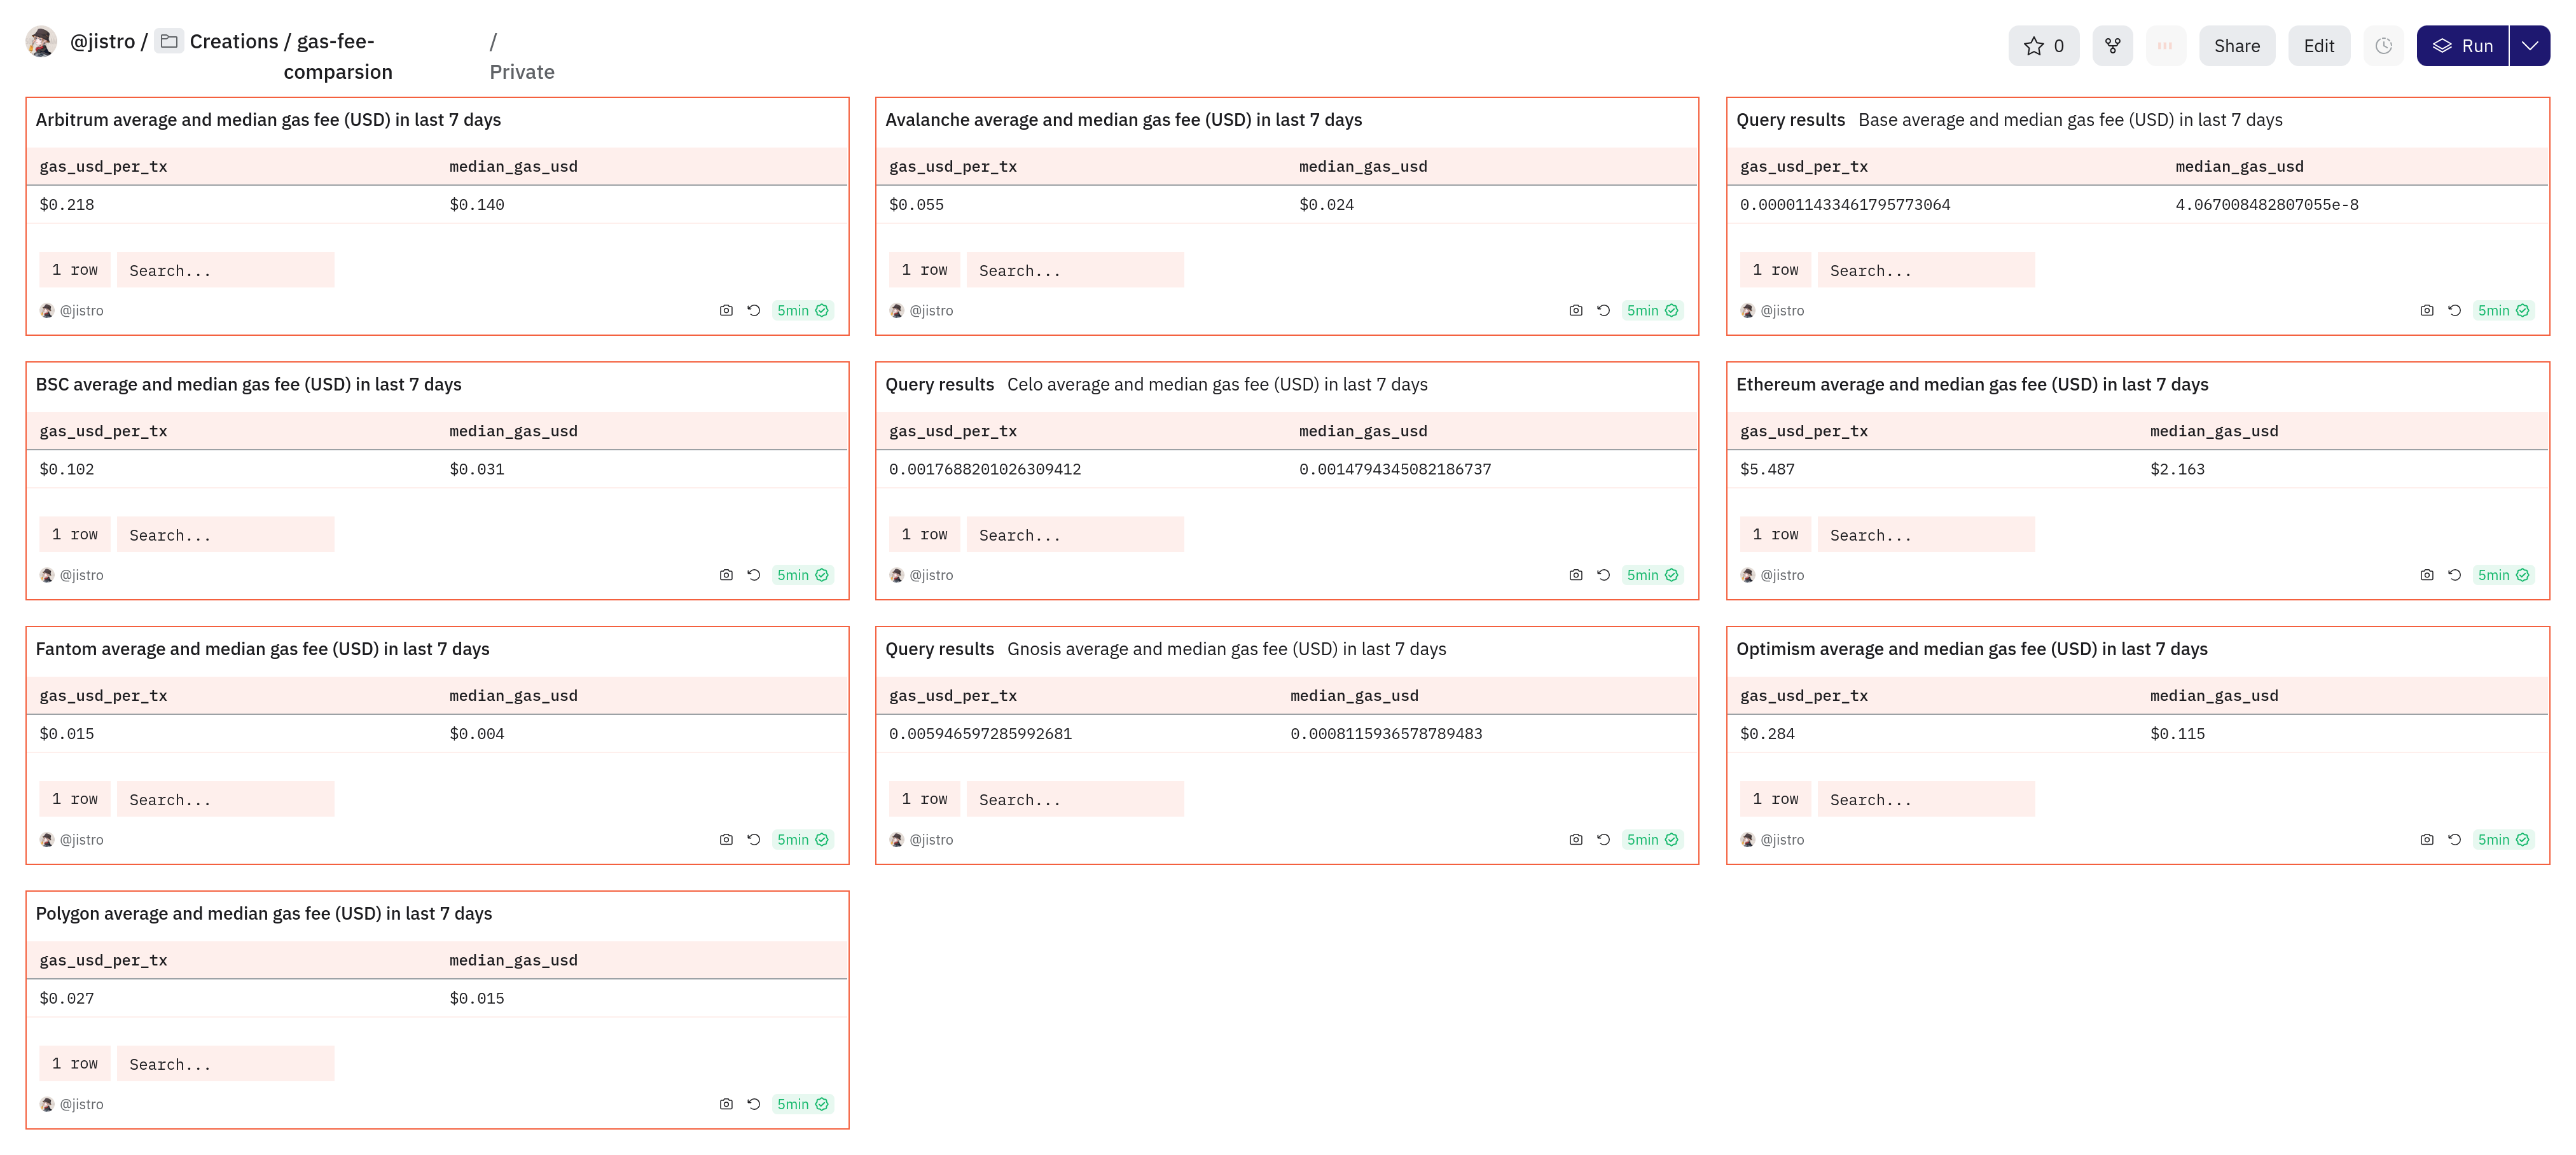
\includegraphics[width=.7\linewidth]{img/gasFeeComp}
	\caption{Comparison of Gas Fees \cite{jistro_gas_2024}}
	\label{fig:gasfeecomp}
\end{figure}
\pagebreak

\subsection{Transaction Per Second and Block Time Data}

For this information, we rely on Chainspect data, retrieved on January 3, 2024, utilizing the Max Recorded Transactions Per Second (Tx/s) and Block Time data \cite{noauthor_technical_nodate}. As seen in Table \ref{tab:TpsAndBT}, the fastest in block time is Arbitrum one, while the highest Tx/s is observed on BNB Chain.

\begin{table}[H]
	\centering
	\begin{tabular}{lll}
		Chain               & Tx/s   & Block time \\
		Arbitrum one        & 97    & 0.27s      \\
		Avalanche (C-Chain) & 682   & 2.03s      \\
		Base                & 385   & 2s         \\
		BNB Chain           & 2,104 & 3s         \\
		Celo                & 454   & 5s         \\
		Ethereum            & 617   & 12s        \\
		Fantom              & 350   & 1.67s      \\
		Gnosis              & 156   & 5.61s      \\
		Optimism            & 242   & 2s         \\
		Polygon             & 673   & 2.13s     
	\end{tabular}
	\caption{Max Recorded Transactions Per Second (Tx/s) and Block Time Data.}
	\label{tab:TpsAndBT}
\end{table}


\begin{table}[H]
	\tiny
	\centering
	\begin{tabular}{|c|c|c|c|c|c|c|c|}
		\hline
		Chain name & \makecell{Median gas \\ fee cost (USD)}  & Tx/s & Block time & Block finality & \makecell{Cross-chain\\ solutions} & \makecell{Optimistic \\ Rollups} & Has Fraud Proof \\ \hline
		
		Gnosis & \cellcolor[RGB]{0,255,0}\$0.0008 & \cellcolor[RGB]{255,100,0}156 & \cellcolor[RGB]{255,50,0}5.61s  & \cellcolor[RGB]{130,255,10}5 seconds \cite{murdock_deep_2022}  & 
\includegraphics[width=0.03\linewidth]{img/logoLayerZero}
		
\includegraphics[width=0.03\linewidth]{img/logoAxelarOPA} 
\includegraphics[width=0.03\linewidth]{img/logoHyperlane} 
\includegraphics[width=0.03\linewidth]{img/logoCCIP} & & \\ \hline
		
		Celo & \cellcolor[RGB]{130,255,10}\$0.0014 & \cellcolor[RGB]{200,255,0}454 & \cellcolor[RGB]{255,100,0}5s  & \cellcolor[RGB]{130,255,10}5 seconds \cite{marek_you_2020} & 
\includegraphics[width=0.03\linewidth]{img/logoLayerZero} 
\includegraphics[width=0.03\linewidth]{img/logoAxelar} 
\includegraphics[width=0.03\linewidth]{img/logoHyperlane} 
\includegraphics[width=0.03\linewidth]{img/logoCCIP} & & \\ \hline
		
		Fantom & \cellcolor[RGB]{100,255,100}\$0.004 & \cellcolor[RGB]{255,150,0}350 & \cellcolor[RGB]{100,255,100}1.67s  & \cellcolor[RGB]{100,255,100}2 seconds \cite{_v_khatibi_how_2023} & 
\includegraphics[width=0.03\linewidth]{img/logoLayerZero} 
\includegraphics[width=0.03\linewidth]{img/logoAxelar}
		
\includegraphics[width=0.03\linewidth]{img/logoHyperlaneOPA} 
\includegraphics[width=0.03\linewidth]{img/logoCCIPOPA} & & \\ \hline
		
		Polygon & \cellcolor[RGB]{150,255,100}\$0.015  & \cellcolor[RGB]{130,255,10}673 & \cellcolor[RGB]{255,200,0}2.13s & \cellcolor[RGB]{255,100,0}5 minutes \cite{idex_polygon_nodate} & 
\includegraphics[width=0.03\linewidth]{img/logoLayerZero} 
\includegraphics[width=0.03\linewidth]{img/logoAxelar} 
\includegraphics[width=0.03\linewidth]{img/logoHyperlane} 
\includegraphics[width=0.03\linewidth]{img/logoCCIP} & & \\ \hline	
		
		Avalanche (C-Chain) & \cellcolor[RGB]{200,255,0}\$0.024  & \cellcolor[RGB]{100,255,100}682 & \cellcolor[RGB]{150,255,100}2.03s & \cellcolor[RGB]{0,255,0}1 second \cite{asim_time_nodate} & 
\includegraphics[width=0.03\linewidth]{img/logoLayerZero} 
\includegraphics[width=0.03\linewidth]{img/logoAxelar}  
\includegraphics[width=0.03\linewidth]{img/logoHyperlane}  
\includegraphics[width=0.03\linewidth]{img/logoCCIP} & & \\ \hline
		
		BNB Chain & \cellcolor[RGB]{255,200,0}\$0.031 & \cellcolor[RGB]{0,255,0}2,104 & \cellcolor[RGB]{255,150,0}3s  & \cellcolor[RGB]{150,255,100}45 seconds \cite{bnb_chain_coming_nodate} & 
\includegraphics[width=0.03\linewidth]{img/logoLayerZero} 
\includegraphics[width=0.03\linewidth]{img/logoAxelar} 
\includegraphics[width=0.03\linewidth]{img/logoHyperlane} 
\includegraphics[width=0.03\linewidth]{img/logoCCIP} & & \\ \hline
		
		Optimism &  \cellcolor[RGB]{255,150,0}\$0.115 & \cellcolor[RGB]{255,50,0}242 & \cellcolor[RGB]{130,255,10}2s & \cellcolor[RGB]{255,0,0}7 days\cite{optimism_understanding_nodate}        & 
\includegraphics[width=0.03\linewidth]{img/logoLayerZero} 
\includegraphics[width=0.03\linewidth]{img/logoAxelar} 
\includegraphics[width=0.03\linewidth]{img/logoHyperlane} 
\includegraphics[width=0.03\linewidth]{img/logoCCIP} & 
\includegraphics[width=0.03\linewidth]{img/check} & \makecell{currently undergoing \\ major redevelopment\cite{optimism_fault_nodate}} \\ \hline
		
		Arbitrum one & \cellcolor[RGB]{255,100,0}\$0.140 & \cellcolor[RGB]{255,0,0}97 & \cellcolor[RGB]{0,255,0}0.27s & \cellcolor[RGB]{255,0,0}7 days\cite{arbitrum_frequently_2023} & 
\includegraphics[width=0.03\linewidth]{img/logoLayerZero} 
\includegraphics[width=0.03\linewidth]{img/logoAxelar} 
\includegraphics[width=0.03\linewidth]{img/logoHyperlane} 
\includegraphics[width=0.03\linewidth]{img/logoCCIP} & 
\includegraphics[width=0.03\linewidth]{img/check} & yes  \cite{arbitrum_fraud_2023} \\ \hline
		
		
		Base & \cellcolor[RGB]{255,50,0}\$1.3381 & \cellcolor[RGB]{255,200,0}385 & \cellcolor[RGB]{130,255,10}2s  & \cellcolor[RGB]{255,0,0}7 days\cite{optimism_understanding_nodate} & 
\includegraphics[width=0.03\linewidth]{img/logoLayerZero} 
\includegraphics[width=0.03\linewidth]{img/logoAxelar} 
\includegraphics[width=0.03\linewidth]{img/logoHyperlane} 
\includegraphics[width=0.03\linewidth]{img/logoCCIP} & 
\includegraphics[width=0.03\linewidth]{img/check} & \makecell{currently undergoing \\ major redevelopment\cite{optimism_fault_nodate}} \\  \hline
		
		Ethereum & \cellcolor[RGB]{255,0,0}\$2.163 & \cellcolor[RGB]{150,255,100}617 & \cellcolor[RGB]{255,0,0}12s  & \cellcolor[RGB]{255,50,0}16 minutes \cite{bnb_chain_coming_nodate} & 
\includegraphics[width=0.03\linewidth]{img/logoLayerZero} 
\includegraphics[width=0.03\linewidth]{img/logoAxelar}  
\includegraphics[width=0.03\linewidth]{img/logoHyperlane} 
\includegraphics[width=0.03\linewidth]{img/logoCCIP} & & \\ \hline
		
	\end{tabular}
	\caption{Comparative chain Data.}
	\label{tab:TableChain}
\end{table}

\subsection{Transaction Data After EIP-4844}

On March 13, 2024, the Dencun network upgrade was activated on the Ethereum mainnet network alongside EIP-4844, also known as Proto-Danksharding \cite{protocol_support_team_dencun_2024}.

Proto-danksharding (EIP-4844) is a proposal that introduces a new transaction type called "blob-carrying transaction" to the Ethereum network. These transactions carry additional data blobs of around 125 kB, which are much cheaper than regular calldata but not accessible to the EVM execution. While validators still need to download full blob data, the bandwidth is limited to 1 MB per slot instead of 16 MB. This provides some scalability gains without full sharding implementation. Proto-danksharding lays the groundwork for Danksharding by introducing necessary transaction formats and verification rules \cite{buterin_proto-danksharding_nodate}.
EIP-4844 helps layer 2 rollup solutions reduce gas fees by enabling more efficient data storage and processing through the introduction of blob-carrying transactions.

To compare the cost of transactions on layer 2 chains before and after the EIP-4844 upgrade, we include the median gas fee cost for both scenarios in Table \ref{tab:EIP4844Table}. This quantifies the impact of the new transaction type on gas fees and demonstrates the cost savings provided by the more efficient data handling mechanisms introduced by EIP-4844.

\begin{table}[H]
	\centering
	\begin{tabular}{lll}
		L2 OP Chain         & Before EIP-4844 fee (USD)  &  After EIP-4844 fee (USD) \cite{l2beat_onchain_nodate}  \\
		Arbitrum one        & \$0.140    & \$0.0077       \\
		Base                & \$1.3381   & \$0.0058        \\
		Optimism            & \$0.115    & \$0.0125        \\
	\end{tabular}
	\caption{Median gas fee cost Before and after EIP-4844.}
	\label{tab:EIP4844Table}
\end{table}

With this information, we can rearrange the new comparative chain data based on gas fee per transaction after EIP-4844, showing the significant reduction in transaction costs enabled by the upgrade.

\begin{table}[H]
	\tiny
	\centering
	\begin{tabular}{|c|c|c|c|c|c|c|c|c|}
		\hline
		Chain name & \makecell{Median gas \\ fee cost \\ post EIP-4844 (USD)}  & \makecell{Median gas \\ fee cost \\ pre EIP-4844 (USD)} & Tx/s & Block time & Block finality & \makecell{Cross-chain\\ solutions} & \makecell{Optimistic \\ Rollups} & Has Fraud Proof \\ \hline
		
		Gnosis & \cellcolor[RGB]{0,255,0}\$0.0008 & \cellcolor[RGB]{0,255,0}\$0.0008 & \cellcolor[RGB]{255,100,0}156 & \cellcolor[RGB]{255,50,0}5.61s  & \cellcolor[RGB]{130,255,10}5 seconds \cite{murdock_deep_2022}  & 
\includegraphics[width=0.03\linewidth]{img/logoLayerZero}
		
\includegraphics[width=0.03\linewidth]{img/logoAxelarOPA} 
\includegraphics[width=0.03\linewidth]{img/logoHyperlane} 
\includegraphics[width=0.03\linewidth]{img/logoCCIP} & & \\ \hline
		
		Celo & \cellcolor[RGB]{130,255,10}\$0.0014 & \cellcolor[RGB]{130,255,10}\$0.0014 & \cellcolor[RGB]{200,255,0}454 & \cellcolor[RGB]{255,100,0}5s  & \cellcolor[RGB]{130,255,10}5 seconds \cite{marek_you_2020} & 
\includegraphics[width=0.03\linewidth]{img/logoLayerZero} 
\includegraphics[width=0.03\linewidth]{img/logoAxelar} \includegraphics[width=0.03\linewidth]{img/logoHyperlane} \includegraphics[width=0.03\linewidth]{img/logoCCIP} & & \\ \hline
		
		Fantom & \cellcolor[RGB]{100,255,100}\$0.004 & \cellcolor[RGB]{100,255,100}\$0.004 & \cellcolor[RGB]{255,150,0}350 & \cellcolor[RGB]{100,255,100}1.67s  & \cellcolor[RGB]{100,255,100}2 seconds \cite{_v_khatibi_how_2023} & \includegraphics[width=0.03\linewidth]{img/logoLayerZero} \includegraphics[width=0.03\linewidth]{img/logoAxelar}
		\includegraphics[width=0.03\linewidth]{img/logoHyperlaneOPA} \includegraphics[width=0.03\linewidth]{img/logoCCIPOPA} & & \\ \hline
		
		Base & \cellcolor[RGB]{150,255,100}\$0.0058 & \cellcolor[RGB]{255,50,0}\$1.3381 & \cellcolor[RGB]{255,200,0}385 & \cellcolor[RGB]{130,255,10}2s  & \cellcolor[RGB]{255,0,0}7 days\cite{optimism_understanding_nodate} & \includegraphics[width=0.03\linewidth]{img/logoLayerZero} \includegraphics[width=0.03\linewidth]{img/logoAxelar} \includegraphics[width=0.03\linewidth]{img/logoHyperlane} \includegraphics[width=0.03\linewidth]{img/logoCCIP} & \includegraphics[width=0.03\linewidth]{img/check} & \makecell{currently undergoing \\ major redevelopment\cite{optimism_fault_nodate}} \\  \hline		
		
		Arbitrum one & \cellcolor[RGB]{200,255,0}\$0.0077 & \cellcolor[RGB]{255,100,0}\$0.140 & \cellcolor[RGB]{255,0,0}97 & \cellcolor[RGB]{0,255,0}0.27s & \cellcolor[RGB]{255,0,0}7 days\cite{arbitrum_frequently_2023} & \includegraphics[width=0.03\linewidth]{img/logoLayerZero} \includegraphics[width=0.03\linewidth]{img/logoAxelar} \includegraphics[width=0.03\linewidth]{img/logoHyperlane} \includegraphics[width=0.03\linewidth]{img/logoCCIP} & \includegraphics[width=0.03\linewidth]{img/check} & yes  \cite{arbitrum_fraud_2023} \\ \hline
		
		Optimism &  \cellcolor[RGB]{255,200,0}\$0.0125 & \cellcolor[RGB]{255,150,0}\$0.115 & \cellcolor[RGB]{255,50,0}242 & \cellcolor[RGB]{130,255,10}2s & \cellcolor[RGB]{255,0,0}7 days\cite{optimism_understanding_nodate}        & \includegraphics[width=0.03\linewidth]{img/logoLayerZero} \includegraphics[width=0.03\linewidth]{img/logoAxelar} \includegraphics[width=0.03\linewidth]{img/logoHyperlane} \includegraphics[width=0.03\linewidth]{img/logoCCIP} & \includegraphics[width=0.03\linewidth]{img/check} & \makecell{currently undergoing \\ major redevelopment\cite{optimism_fault_nodate}} \\ \hline
		
		Polygon & \cellcolor[RGB]{255,150,0}\$0.015  & \cellcolor[RGB]{150,255,100}\$0.015  & \cellcolor[RGB]{130,255,10}673 & \cellcolor[RGB]{255,200,0}2.13s & \cellcolor[RGB]{255,100,0}5 minutes \cite{idex_polygon_nodate} & \includegraphics[width=0.03\linewidth]{img/logoLayerZero} \includegraphics[width=0.03\linewidth]{img/logoAxelar} \includegraphics[width=0.03\linewidth]{img/logoHyperlane} \includegraphics[width=0.03\linewidth]{img/logoCCIP} & & \\ \hline	
		
		Avalanche (C-Chain) & \cellcolor[RGB]{255,100,0}\$0.024 & \cellcolor[RGB]{200,255,0}\$0.024  & \cellcolor[RGB]{100,255,100}682 & \cellcolor[RGB]{150,255,100}2.03s & \cellcolor[RGB]{0,255,0}1 second \cite{asim_time_nodate} & \includegraphics[width=0.03\linewidth]{img/logoLayerZero} \includegraphics[width=0.03\linewidth]{img/logoAxelar}  \includegraphics[width=0.03\linewidth]{img/logoHyperlane}  \includegraphics[width=0.03\linewidth]{img/logoCCIP} & & \\ \hline
		
		BNB Chain & \cellcolor[RGB]{255,50,0}\$0.031 & \cellcolor[RGB]{255,200,0}\$0.031 & \cellcolor[RGB]{0,255,0}2,104 & \cellcolor[RGB]{255,150,0}3s  & \cellcolor[RGB]{150,255,100}45 seconds \cite{bnb_chain_coming_nodate} & \includegraphics[width=0.03\linewidth]{img/logoLayerZero} \includegraphics[width=0.03\linewidth]{img/logoAxelar} \includegraphics[width=0.03\linewidth]{img/logoHyperlane} \includegraphics[width=0.03\linewidth]{img/logoCCIP} & & \\ \hline
		
		
		Ethereum & \cellcolor[RGB]{255,0,0}\$2.163 & \cellcolor[RGB]{255,0,0}\$2.163 & \cellcolor[RGB]{150,255,100}617 & \cellcolor[RGB]{255,0,0}12s  & \cellcolor[RGB]{255,50,0}16 minutes \cite{bnb_chain_coming_nodate} & \includegraphics[width=0.03\linewidth]{img/logoLayerZero} \includegraphics[width=0.03\linewidth]{img/logoAxelar}  \includegraphics[width=0.03\linewidth]{img/logoHyperlane} \includegraphics[width=0.03\linewidth]{img/logoCCIP} & & \\ \hline
		
	\end{tabular}
	\caption{Comparative chain Data Post EIP-4844.}
	\label{tab:TableChainDank}
\end{table}




\newpage
\bibliography{citations}

\end{document}